%beamer

% Comment/uncomment this line to toggle handout mode
\newcommand{\handout}{}

%% Beamer-Klasse im korrekten Modus
\ifdefined \handout
\documentclass[handout]{beamer} % Handout mode
\else
\documentclass{beamer}
\fi

%% UTF-8-Encoding
\usepackage[utf8]{inputenc}

\input{../framework/gbi-macros}
\usepackage[blue]{../framework/thwregex}
\usepackage{environ}
\usepackage{bm}
\usepackage{calc}
\usepackage{varwidth}
\usepackage{wasysym}
\usepackage{mathtools}


% Das ist der KIT-Stil
%\usepackage{../TutTexbib/beamerthemekit}
\usepackage[deutsch,titlepage0]{../framework/KIT/beamerthemeKITmod}
\TitleImage[width=\titleimagewd]{../figures/titlepage.jpg}
%\usetheme[deutsch,titlepage0]{KIT}

% Include PDFs
\usepackage{pdfpages}

% Libertine font (Original GBI font)
\usepackage{libertine}
%\renewcommand*\familydefault{\sfdefault}  %% Only if the base font of the document is to be sans serif

% Nicer math symbols
\usepackage{eulervm}
%\usepackage{mathpazo}
\renewcommand\ttdefault{cmtt} % Computer Modern typewriter font, see lecture slides.

\usepackage{csquotes}

%%%%%%

%% Schönere Schriften
\usepackage[TS1,T1]{fontenc}

%% Bibliothek für Graphiken
\usepackage{graphicx}

%% der wird sowieso in jeder Datei gesetzt
\graphicspath{{../figures/}}

%% Anzeigetiefe für Inhaltsverzeichnis: 1 Stufe
\setcounter{tocdepth}{1}

%% Hyperlinks
\usepackage{hyperref}
% I don't know why, but this works and only includes sections and NOT subsections in the pdf-bookmarks.
\hypersetup{bookmarksdepth=subsection} 

%\usepackage{lmodern}
\usepackage{colortbl}
\usepackage[absolute,overlay]{textpos}
\usepackage{listings}
\usepackage{forloop}
%\usepackage{algorithmic} % PseudoCode package 

\usepackage{tikz}
\usetikzlibrary{matrix}
\usetikzlibrary{arrows.meta}
\usetikzlibrary{automata}
\usetikzlibrary{tikzmark}
\usetikzlibrary{positioning}

% Why has no-one come up with this yet? I mean, seriously. -.-
\tikzstyle{loop below right} = [loop, out=-60,in=-30, looseness=7]
\tikzstyle{loop below left} = [loop, out=-150,in=-120, looseness=7]
\tikzstyle{loop above right} = [loop, out=60,in=30, looseness=7]
\tikzstyle{loop above left} = [loop, out=150,in=120, looseness=7]
\tikzstyle{loop right below} = [loop below right]
\tikzstyle{loop left below} = [loop below left]
\tikzstyle{loop right above} = [loop above right]
\tikzstyle{loop left above} = [loop above left]

% Needed for gbi-macros
\usepackage{xspace}

%%%%%%

%% Verbatim
\usepackage{moreverb}

%%%%%%%%%%%%%%%%%%%%%%%%%%%%%%%%%%%% Copy end

%% Tabellen
\usepackage{array}
\usepackage{multicol}
\usepackage{hhline}

%% Bibliotheken für viele mathematische Symbole
\usepackage{amsmath, amsfonts, amssymb}

%% Deutsche Silbentrennung und Beschriftungen
\usepackage[ngerman]{babel}

\usepackage{kbordermatrix}

% kbordermatrix settings
\renewcommand{\kbldelim}{(} % Left delimiter
\renewcommand{\kbrdelim}{)} % Right delimiter

\input{../config.tex}



% define custom \handout command flag if handout mode is toggled  #DirtyAsHellButWell...
\only<beamer:0>{\def\handout{}} %beamer:0 == handout mode

\newcommand{\R}{\mathbb{R}}
\newcommand{\N}{\mathbb{N}}
\newcommand{\Z}{\mathbb{Z}}
\newcommand{\Q}{\mathbb{Q}}
\newcommand{\BB}{\mathbb{B}}
\newcommand{\C}{\mathbb{C}}
\newcommand{\K}{\mathbb{K}}
\newcommand{\G}{\mathbb{G}}
\newcommand{\nullel}{\mathcal{O}}
\newcommand{\einsel}{\mathds{1}}
\newcommand{\Pot}{\mathcal{P}}
\renewcommand{\O}{\text{O}}

\def\word#1{\hbox{\textcolor{blue}{\texttt{#1}}}}
\let\literal\word
\def\mword#1{\hbox{\textcolor{blue}{$\mathtt{#1}$}}}  % math word
\def\sp{\scalebox{1}[.5]{\textvisiblespace}}
\def\wordsp{\word{\sp}}

%\newcommand{\literal}[1]{\textcolor{blue}{\texttt{#1}}}
\newcommand{\realTilde}{\textasciitilde \ }
\newcommand{\setsize}[1]{\ensuremath{\left\lvert #1 \right\rvert}}
\newcommand{\size}[1]{\setsize{#1}}  % Shame on you, TeXStudio...
\newcommand{\set}[1]{\left\{#1\right\}}
\newcommand{\tuple}[1]{\left(#1\right)}
\newcommand{\normalvar}[1]{\text{$#1$}}

% Modified by DJ
\let\oldemptyset\emptyset
\let\emptyset\varnothing % proper emptyset

\newcommand{\boder}{\ensuremath{\mathbin{\textcolor{blue}{\vee}}}\xspace}
\newcommand{\bund}{\ensuremath{\mathbin{\textcolor{blue}{\wedge}}}\xspace}
\newcommand{\bimp}{\ensuremath{\mathrel{\textcolor{blue}{\to}}}\xspace}
\newcommand{\bgdw}{\ensuremath{\mathrel{\textcolor{blue}{\leftrightarrow}}}\xspace}
\newcommand{\bnot}{\ensuremath{\textcolor{blue}{\neg}}\xspace}
\newcommand{\bone}{\ensuremath{\textcolor{blue}{1}}\text{}}
\newcommand{\bzero}{\ensuremath{\textcolor{blue}{0}}\text{}}
\newcommand{\bleftBr}{\ensuremath{\textcolor{blue}{\texttt{(}}}\text{}}
\newcommand{\brightBr}{\ensuremath{\textcolor{blue}{\texttt{)}}}\text{}}

% Fix of \b... commands:

\renewcommand{\boder}{\alor}
\renewcommand{\bund}{\aland}
\renewcommand{\bimp}{\alimpl}
\renewcommand{\bgdw}{\aleqv}
\renewcommand{\bnot}{\alnot}
\renewcommand{\bleftBr}{\alka}
\renewcommand{\brightBr}{\alkz}
\newcommand{\alA}{\word A}
\newcommand{\alB}{\word B}
\newcommand{\alC}{\word C}

\newcommand{\plB}{\plfoo{B}}
\newcommand{\plE}{\plfoo{E}}

\newcommand{\summe}[2]{\sum\limits_{#1}^{#2}}
\newcommand{\limes}[1]{\lim\limits_{#1}}

%\newcommand{\numpp}{\advance \value{weeknum} by -2 \theweeknum \advance \value{weeknum} by 2}
%\newcommand{\nump}{\advance \value{weeknum} by -1 \theweeknum \advance \value{weeknum} by 1}

\newcommand{\mycomment}[1]{}
\newcommand{\Comment}[1]{}

%% DISCLAIMER START 
% It is INSANELY IMPORTANT NOT TO DO THIS OUTSIDE BEAMER CLASS! IN ARTCILE DOCUMENTS, THIS IS VERY LIKELY TO BUG AROUND!
\makeatletter%
\@ifclassloaded{beamer}%
{
	% TODO 
	% no time... later.   (= never -.-)
	% redefine section to ignore multiple \section calls with the same title
}%
{
	\errmessage{ERROR: section command redefinition outside of beamer class document! Please contact the author of this code or read the F-ing disclaimer.}
}%
\makeatother%
%% DISCLAIMER END

\newcounter{abc}
\newenvironment{alist}{
  \begin{list}{(\alph{abc})}{
      \usecounter{abc}\setlength{\leftmargin}{8mm}\setlength{\labelsep}{2mm}
    }
}{\end{list}}


\newcommand{\stdarraystretch}{1.20}
\renewcommand{\arraystretch}{\stdarraystretch}  % for proper row spacing in tables

\newcommand{\morescalingdelimiters}{   % for proper \left( \right) typography
	\delimitershortfall=-1pt  
	\delimiterfactor=1
}

\newcommand{\centered}[1]{\vspace{-\baselineskip}\begin{center}#1\end{center}\vspace{-\baselineskip}}

% for \implitem and \item[bla] stuff to look right:
\setbeamercolor*{itemize item}{fg=black}
\setbeamercolor*{itemize subitem}{fg=black}
\setbeamercolor*{itemize subsubitem}{fg=black}

\setbeamercolor*{description item}{fg=black}
\setbeamercolor*{description subitem}{fg=black}
\setbeamercolor*{description subsubitem}{fg=black}

\renewcommand{\qedsymbol}{\textcolor{black}{\openbox}}

\renewcommand{\mod}{\mathop{\textbf{mod}}}
\renewcommand{\div}{\mathop{\textbf{div}}}

\newcommand{\ceil}[1]{\left\lceil#1\right\rceil}
\newcommand{\floor}[1]{\left\lfloor#1\right\rfloor}
\newcommand{\abs}[1]{\left\lvert #1 \right\rvert}
\newcommand{\Matrix}[1]{\begin{pmatrix} #1 \end{pmatrix}}
\newcommand{\braced}[1]{\left\lbrace #1 \right\rbrace}

% "something" placeholder. Useful for repairing spacing of operator sections, like `\sth = 42`.
\def\sth{\vphantom{.}}

\def\fract#1/#2 {\frac{#1}{#2}} % ! Trailing space is crucial!
\def\dfract#1/#2 {\dfrac{#1}{#2}} % ! Trailing space is crucial!

\newcommand{\Mid}{\;\middle|\;}

\let\after\circ



\def\·{\cdot}
\def\*{\cdot}
\def\?>{\ensuremath{\rightsquigarrow}}  % Fuck you, Latex
\def\~~>{\ensuremath{\rightsquigarrow}}  

\newcommand{\tight}[1]{{\renewcommand{\arraystretch}{0.76} #1}}
\newcommand{\stackedtight}[1]{\renewcommand{\arraystretch}{0.76} \begin{matrix} #1 \end{matrix} }
\newcommand{\stacked}[1]{\begin{matrix} #1 \end{matrix} }
\newcommand{\casesl}[1]{\delimitershortfall=0pt  \left\lbrace\hspace{-.3\baselineskip}\begin{array}{ll} #1 \end{array}\right.}
\newcommand{\casesr}[1]{\delimitershortfall=0pt  \left.\begin{array}{ll} #1 \end{array}\hspace{-.3\baselineskip}\right\rbrace}
\newcommand{\caseslr}[1]{\delimitershortfall=0pt  \left\lbrace\hspace{-.3\baselineskip}\begin{array}{ll} #1 \end{array}\hspace{-.3\baselineskip}\right\rbrace}

\def\q#1uad{\ifnum#1=0\relax\else\quad\q{\the\numexpr#1-1\relax}uad\fi}
% e.g. \q1uad = \quad, \q2uad = \qquad etc.

\newcommand{\qqquad}{\q3uad}
\newcommand{\minusquad}{\hspace{-1em}}

%% Placeholder utils
% \§{#1}   Saves #1 as placeholder and prints it
% \.       Prints an \hphantom with the size of the recalled placeholder.
\def\indentstring{}
\def\§#1{\def\indentstring{#1}#1}
\def\.{{$\hphantom{\text{\indentstring}}$}}
%% Placeholder utils end

\newcommand{\impl}{\ifmmode\ensuremath{\mskip\thinmuskip\Rightarrow\mskip\thinmuskip}\else$\Rightarrow$\fi\xspace}
\newcommand{\Impl}{\ifmmode\implies\else$\Longrightarrow$\fi\xspace}

\newcommand{\derives}{\Rightarrow}

\newcommand{\gdw}{\ifmmode\mskip\thickmuskip\Leftrightarrow\mskip\thickmuskip\else$\Leftrightarrow$\fi\xspace}
\newcommand{\Gdw}{\ifmmode\iff\else$\Longleftrightarrow$\fi\xspace}

% Legacy code from the algo tutorial slides. Perhaps useful. Try with care.
\mycomment{
	\newcommand{\impl}{\ifmmode\ensuremath{\mskip\thinmuskip\Rightarrow\mskip\thinmuskip}\else$\Rightarrow$\xspace\fi}  
	\newcommand{\Impl}{\ifmmode\implies\else$\Longrightarrow$\xspace\fi}
	
	\newcommand{\gdw}{\ifmmode\mskip\thickmuskip\Leftrightarrow\mskip\thickmuskip\else$\Leftrightarrow$\xspace\fi}
	\newcommand{\Gdw}{\ifmmode\iff\else$\Longleftrightarrow$\xspace\fi}
}
	
\newcommand{\gdwdef}{\ifmmode\mskip\thickmuskip:\Leftrightarrow\mskip\thickmuskip\else:$\Leftrightarrow$\xspace\fi}
\newcommand{\Gdwdef}{\ifmmode\mskip\thickmuskip:\Longleftrightarrow\mskip\thickmuskip\else:$\Longleftrightarrow$\xspace\fi}

\newcommand{\symbitemnegoffset}{\hspace{-.5\baselineskip}}
\newcommand{\implitem}{\item[\impl\symbitemnegoffset]}
\newcommand{\Implitem}{\item[\Impl\symbitemnegoffset]}


\newcommand{\forcenewline}{\mbox{}\\}

\newcommand{\bfalert}[1]{\textbf{\alert{#1}}}
\let\elem\in   % I'm a Haskell freak. Don't judge me. :P


\def\|#1|{\text{\normalfont #1}}  % | steht für senkrecht (anstatt kursiv wie sonst im math mode)


% proper math typography
\newcommand{\functionto}{\longrightarrow}
\renewcommand{\geq}{\geqslant}
\renewcommand{\leq}{\leqslant}
\let\oldsubset\subset
\renewcommand{\subset}{\subseteq} % for all idiots out there using subset

\newenvironment{threealign}{%
	\[
	\begin{array}{r@{\ }c@{\ }l}
}{%
	\end{array}	
	\]
}

\newcommand{\concludes}{ \\ \hline  }
\newcommand{\deduction}[1]{
	\begin{varwidth}{.8\linewidth}
		\begin{tabular}{>{$}c<{$}}
			#1
		\end{tabular}
	\end{varwidth}	
}

\definecolor{hoareorange}{rgb}{1,.85,.6}
\newcommand{\hoareassert}[1]{\setlength{\fboxsep}{1pt}\setlength{\fboxrule}{-1.4pt}\fcolorbox{white}{hoareorange}{\ensuremath{\{\;#1\;\}}}\setlength\fboxrule{\defaultfboxrule}\setlength{\fboxsep}{3pt}}

\newcommand{\mailto}[1]{\href{mailto:#1}{{\textcolor{blue}{\underline{#1}}}}}
\newcommand{\urlnamed}[2]{\href{#2}{\textcolor{blue}{\underline{#1}}}}
\renewcommand{\url}[1]{\urlnamed{#1}{#1}}

\newcommand{\hanging}{\hangindent=0.7cm}
\newcommand{\indented}{\hanging}


% \hstretchto prints #2 left-aligned into a box of the width of #1
\def\hstretchto#1#2{%
	\mbox{}\vphantom{#2}\rlap{#2}\hphantom{#1}%
}

\def\vstretchto#1#2{%
	\mbox{}\hphantom{#2}\smash{#2}\vphantom{#1}%
}

% \hstretchtocentered prints #2 centered into a box of the width of #1
\def\hstretchtocentered#1#2{%
	\mbox{}\vphantom{#2}\scalebox{0.5}{\hphantom{#1}}\clap{#2}\scalebox{0.5}{\hphantom{#1}}%
}

% vertical centering
\newcommand{\vertcenter}[1]{%
	\ensuremath{\vcenter{\hbox{#1}}}%
}


%requires \thisyear to be defined (s. config.tex)!
\edef\nextyear{\the\numexpr\thisyear+1\relax}


% --- \frameheight constant ---
\newlength\fullframeheight
\newlength\framewithtitleheight
\setlength\fullframeheight{.92\textheight}
\setlength\framewithtitleheight{.86\textheight}

\newlength\frameheight
\setlength\frameheight{\fullframeheight}

\let\frametitleentry\relax
\let\oldframetitle\frametitle
\def\newframetitle#1{\global\def\frametitleentry{#1}\if\relax\frametitleentry\relax\else\setlength\frameheight{\framewithtitleheight}\fi\oldframetitle{#1}}
\let\frametitle\newframetitle

\def\newframetitleoff{\let\frametitle\oldframetitle}
\def\newframetitleon{\let\frametitle\newframetitle}
% --- \frameheight constant end ---

\newcommand{\fakeframetitle}[1]{%
	\vspace{-2.05\baselineskip}%
	{\Large \textbf{#1}} \\%
	\smallskip
}



\newenvironment{headframe}{\Huge THIS IS AN ERROR. PLEASE CONTACT THE ADMIN OF THIS TEX CODE. (headframe env def failed)}{}
\RenewEnviron{headframe}[1][]{
	\begin{frame}\frametitle{\ }
		\centering
		\Huge\textbf{\textsc{\BODY} \\
		}
		\Large {#1}
		\frametitle{\ }
	\end{frame}
}


\makeatletter
% Provides color if undefined.
\newcommand{\colorprovide}[2]{%
	\@ifundefinedcolor{#1}{\colorlet{#1}{#2}}{}}
\makeatother


\colorprovide{lightred}{red!30}
\colorprovide{lightgreen}{green!40}
\colorprovide{lightyellow}{yellow!50}
\colorprovide{lightblue}{blue!10}
\colorprovide{beamerlightred}{lightred}
\colorprovide{beamerlightgreen}{lightgreen}
\colorprovide{beamerlightyellow}{lightyellow}
\colorprovide{beamerlightblue}{lightblue}
\colorprovide{fullred}{red!60}
\colorprovide{fullgreen}{green}
\definecolor{darkred}{RGB}{115,48,38}
\definecolor{darkgreen}{RGB}{48,115,38}
\definecolor{darkyellow}{RGB}{100,100,0}

\only<handout:0>{\colorlet{adaptinglightred}{beamerlightred}}
\only<handout:0>{\colorlet{adaptinglightgreen}{beamerlightgreen}}
\only<handout:0>{\colorlet{adaptinglightyellow}{beamerlightyellow}}
\only<handout:0>{\colorlet{adaptinglightblue}{beamerlightblue}}
\only<beamer:0>{\colorlet{adaptinglightred}{lightred}}
\only<beamer:0>{\colorlet{adaptinglightgreen}{lightgreen}}
\only<beamer:0>{\colorlet{adaptinglightyellow}{lightyellow}}
\only<beamer:0>{\colorlet{adaptinglightblue}{lightblue}}
\only<handout:0>{\colorlet{adaptingred}{lightred}}
\only<beamer:0>{\colorlet{adaptingred}{fullred}}
\only<handout:0>{\colorlet{adaptinggreen}{lightgreen}}
\only<beamer:0>{\colorlet{adaptinggreen}{fullgreen}}



\newcommand{\TrueQuestion}[1]{
	\TrueQuestionE{#1}{}
}

\newcommand{\YesQuestion}[1]{
	\YesQuestionE{#1}{}
}

\newcommand{\FalseQuestion}[1]{
	\FalseQuestionE{#1}{}
}

\newcommand{\NoQuestion}[1]{
	\NoQuestionE{#1}{}
}

\newcommand{\DependsQuestion}[1]{
	\DependsQuestionE{#1}{}
}

\newcommand{\QuestionVspace}{\vspace{4pt}}
\newcommand{\QuestionParbox}[1]{\begin{varwidth}{.85\linewidth}#1\end{varwidth}}
\newcommand{\ExplanationParbox}[1]{\begin{varwidth}{.97\linewidth}#1\end{varwidth}}
\colorlet{questionlightgray}{gray!23}
\let\defaultfboxrule\fboxrule

% #1: bg color
% #2: fg color short answer
% #3: short answer text
% #4: question
% #5: explanation
\newcommand{\GenericQuestion}[5]{
	\setlength\fboxrule{2pt}
	\only<+|handout:0>{\hspace{-2pt}\fcolorbox{white}{questionlightgray}{\QuestionParbox{#4} \quad\textbf{?}}}
	\visible<+->{\hspace{-2pt}\fcolorbox{white}{#1}{\QuestionParbox{#4} \quad\textbf{\textcolor{#2}{#3}}} \if\relax#5\relax\else\ExplanationParbox{#5}\fi} \\
	\setlength\fboxrule{\defaultfboxrule}
}

% #1: Q text
% #2: Explanation
\newcommand{\TrueQuestionE}[2]{
	\GenericQuestion{adaptinglightgreen}{darkgreen}{Wahr.}{#1}{#2}
}

% #1: Q text
% #2: Explanation
\newcommand{\YesQuestionE}[2]{
	\GenericQuestion{adaptinglightgreen}{darkgreen}{Ja.}{#1}{#2}
}

% #1: Q text
% #2: Explanation
\newcommand{\FalseQuestionE}[2]{
	\GenericQuestion{adaptinglightred}{darkred}{Falsch.}{#1}{#2}
}

% #1: Q text
% #2: Explanation
\newcommand{\NoQuestionE}[2]{
	\GenericQuestion{adaptinglightred}{darkred}{Nein.}{#1}{#2}
}

% #1: Q text
% #2: Explanation
\newcommand{\DependsQuestionE}[2]{
	\GenericQuestion{adaptinglightyellow}{darkyellow}{Je nachdem!}{#1}{#2}
}

% #1: Q text
% #2: Answer
\newcommand{\ContentQuestion}[2]{
	\GenericQuestion{adaptinglightblue}{black}{\minusquad}{#1}{#2}
}

\ifnum\thisyear=2021 \else \errmessage{Old ILIAS link inside preamble. Please update.} \fi

\newcommand{\ILIAS}{\urlnamed{ILIAS}{\myILIASurl}\xspace}
\newcommand{\Klausurtermin}{\myKlausurtermin\xspace}

\newcommand{\Socrative}{\ifdefined\mysocrativeroom \only<handout:0>{socrative.com $\quad \~~> \quad $ Student login \\ Raumname:  \mysocrativeroom\\ \medskip}\else\fi}

\newcommand{\thasse}[1]{
	\ifdefined\ThassesTut #1\xspace \else\fi
}
\newcommand{\daniel}[1]{
	\ifdefined\DanielsTut #1\xspace \else\fi
}
\newcommand{\thassedaniel}[2]{\ifdefined\ThassesTut #1\else\ifdefined\DanielsTut #2\fi\fi\xspace}

\ifdefined\ThassesTut \ifdefined\DanielsTut \errmessage{ERROR: Both ThassesTut and DanielsTut flags are set. This is most likely an error. Please check your config.tex file.} \else \fi \else \ifdefined\DanielsTut \else \errmessage{ERROR: Neither ThassesTut  nor DanielsTut flags are set. This is most likely an error. Please check your config.tex file.} \fi\fi

%\newcommand{\sgn}{\text{sgn}}

%%%%%%%%%%%% INHALT %%%%%%%%%%%%%%%%

%% Wochennummer
\newcounter{weeknum}

%% Titelinformationen
\title[GBI-Tutorium \mytutnumber, Woche \theweeknum]{Grundbegriffe der Informatik \\ Tutorium \mytutnumber}

\subtitle{Woche \theweeknum\xspace |\xspace\mydate{\theweeknum} \\ \myname \ \  \normalfont (\mailto{\mymail})}
\author[\myname]{\myname}
\institute{KIT -- Karlsruher Institut für Technologie}
\date{\mydate{\theweeknum}\ }

% Modified, DJ (better safe than sorry)
\AuthorTitleSep{ – }

%% Titel einfügen
\newcommand{\titleframe}{\frame{\titlepage}}

%% Alles starten mit \starttut{X}
\newcommand{\starttut}[1]{\setcounter{weeknum}{#1}\pdfinfo{
		/Author (\myname)
		/Title  (GBI-Tutorium \mytutnumber, Woche \theweeknum)
	}\titleframe\frame{\frametitle{Inhalt}\tableofcontents} \AtBeginSection[]{%
		\begin{frame}{Wo sind wir gerade?}
		\tableofcontents[currentsection]
	\end{frame}\addtocounter{framenumber}{-1}}}


\newcommand{\framePrevEpisode}{
\begin{headframe}
	\mylasttimestext
\end{headframe}
}

\newcommand{\lastframetitled}[6]{
	\frame{\frametitle{#6}
		\vspace{-#2\baselineskip}
		\begin{figure}[H]
			\centering
			\LARGE \textbf{\textsc{#5}} \\
			\vspace{.2\baselineskip}
			\includegraphics[#1]{#3}
			\vspace{-6pt}
			\begin{center}
				\small \url{#4} 
			\end{center}
		\end{figure} 
	}
}

% #1 number
% #2 title 
% #3 vspace (positive) without unit (\baselineskip)
\newcommand{\xkcdframe}[3]{
	\lastframetitled{width=.96\textwidth}{#3}{xkcd/#1}{http://xkcd.com/#1}{}{#2}
}

\newcommand{\xkcdframevert}[3]
{
	\lastframetitled{height=.96\frameheight}{#3}{xkcd/#1}{http://xkcd.com/#1}{}{#2}
}

% #1 number
% #2 title 
% #3 vspace (positive) without unit (\baselineskip)
% #4 \includegraphics[] optional parameters
\newcommand{\xkcdframecustom}[4]
{
	\lastframetitled{#4}{#3}{xkcd/#1}{http://xkcd.com/#1}{}{#2}
}

\newcommand{\slideThanks}{
	\begin{frame}
	\frametitle{Credits}
	\begin{block}{}
		An der Erstellung des Foliensatzes haben mitgewirkt:\\[1em]
		Daniel Jungkind \\
		Thassilo Helmold \\
		Philipp Basler \\
		Nils Braun \\
		Dominik Doerner \\
		Ou Yue \\
		Max Schweikart
	\end{block}
\end{frame}
}

%% Wörter DEPRECATED! DO NOT USE
\newcommand{\code}[1]{$\mathbf{#1}$}

\morescalingdelimiters

\begin{document}
\starttut{2}

\section{Organisatorisches}

\begin{frame}[t]{Änderung Übungsblattabgabe}
	So sollte eure Abgabe aussehen:
	\begin{itemize}
		\item Namen und Matrikelnummer \textbf{beider} Abgabepartner aufs Deckblatt!
		\item Handschriftliche Bearbeitung (Papier oder Tablet mit Ausdruck)
		\item Lesbar schreiben, Rand freilassen!
		\item Übungsblatt \textbf{pünktlich} abgeben!
		\item Abgabe nun in Holzkiste \textbf{vor Raum 016}!
	\end{itemize}
\end{frame}

\mycomment{ % From year 2020, omitted because tutorial dropped because of holiday
	\begin{frame}{Zu Blatt \#1}
		
		Schnitt: \quad \thassedaniel{14.6}{13.7} / 17~P
		
		\begin{itemize}[<+->]
			\item Erstmal: Volle Punktzahl ist utopisch. Fehler macht man, um draus zu lernen – dazu sind ÜBs da
			\item \textbf{Einfachstes} Beispiel für $(A \setminus (B \setminus C)) \setminus D = (A \setminus B) \setminus (C \setminus D)$? \only<beamer:0>{\\ \impl $A = B = C = D = \emptyset$.}
			\item Für eine Menge $A$ ist $\setsize{A + x}$ nicht definiert! \\
			Passt mit euren \textbf{Operatoren} auf: \impl $\setsize{A \cup \set{x}}$
			\item Wenn keine Begründung/Beweis gefordert ist, müsst ihr keinen angeben. („Geben Sie an...“ / „Was ist...“)
			\item Nicht mehrere Alternativen angeben, unter denen ich mir die richtige heraussuchen soll. (That's \emph{your} job!)
			\mycomment{\item \textbf{TACKERN} und \textbf{DECKBLÄTTER}! Sonst \alert{\textbf{null Punkte}}!}
			\daniel{\item Bitte die Aufgabenblätter \textbf{nicht} mitabgeben (Deckblatt reicht), sonst wird mein Stapel so fett. \smiley}
		\end{itemize}
		\thasse{\FalseQuestionE{Ein Beispiel langt als Beweis.}{...bis ein anderes Beispiel herkommt, bei dem es kaputt geht... \\
				\impl eine Behauptung \textbf{widerlegen} geht mit nem Beispiel sehr gut!}}
	\end{frame}
}

\mycomment{  % Keine Zeit... Auch nicht sehr nötig diesmal...
	\begin{frame}[t]{Übungsblätter: Häufige Fehler \daniel{und anderer Kram}}
		
		\TrueQuestionE{Beweise fängt man mit der Behauptung an.}{}
		\FalseQuestionE{Wenn wir $A$ schreiben, ist das immer eine Menge, \\ und $f, g$ sind immer Funktionen.}{Das muss man \textbf{explizit} angeben.}
		\FalseQuestionE{Ein Beispiel langt als Beweis.}{...bis ein anderes Beispiel herkommt, bei dem es kaputt geht... \\
			\impl eine Behauptung \textbf{widerlegen} geht mit nem Beispiel sehr gut!}
		%Mit einem Beispiel kann man eine Behauptung widerlegen, es zeigt aber nicht die Allgemeingültigkeit}
		\FalseQuestionE{$\setsize{M} = M$ für $M \subseteq \N$.}{$\setsize{M}$ ist die \textbf{Anzahl} der Elemente in $M$. Nix mit „Betrag“.}
		
		\medskip
		
		\uncover<9->{Passt auf, was eure Variablen sind und welche Operationen ihr darauf anwenden könnt. Mengen kann man nicht mit $\bund$ und $\boder$ verknüpfen und auch keine \impl dazwischen tun.}
		
	\end{frame}
}


%\begin{frame}{Wahr oder falsch?}
%	\Socrative
%	\TrueQuestionE{$ \setsize{\emptyset} = 0$.}{}
%	\FalseQuestionE{$ \setsize{ \set{\set{}} } = 0$.}{$ \setsize{\set{\set{}}} = \setsize{\set{\emptyset}} = 1$.}
%	\TrueQuestionE{$ \setsize{\set{ 1, \set{2, 3}, 4, \set{5,6,7}}} = 4$.}{$\set{2, 3}$ und $\set{5,6,7}$ sind zwei einzelne Objekte!}
%	\TrueQuestionE{$ \{1, 2\} = \{2, 1\}$.}{}
%	\FalseQuestion{$ (1, 2) = (2, 1)$.}
%	\FalseQuestionE{$ \left(M\cup A\right)\setminus M = A $.}{für z.~B. $ M = A = \{1\}$}
%	%TODO Relationen-Fragen noch? Wenn's im ersten Tut schon vorkam!
%	\visible<12->{
%	\begin{block}{Bemerkungen}
%		Menge / Tupel: Klammern beachten! Einfache Beispiele helfen!
%	\end{block}
%	}
%\end{frame}

\begin{frame}[t]{Mengengleichheit: Aufgabe}
	\begin{itemize}
		\item<1-> Sei $ A, B, C $ beliebige Mengen. Zeigt, dass gilt 
		\begin{align*}
		A \cup (B \cap C) &=  (A \cup B) \cap (A \cup C)
		\end{align*}		 
		\only<2-5>{
			\item<2-5> \textbf{Richtung}: $ A \cup (B \cap C) \subseteq  (A \cup B) \cap (A \cup C) $ 
			\item<3-5> Sei $ x \in A \cup (B \cap C) $.
			\item<4-5> Fall 1: Ist $ x \in A$, so folgt $ x \in A \cup B $ und $ x\in A \cup C$ und damit $  x\in (A \cup B) \cap (A \cup C) $
			\item<5-5> Fall 2 : Ist $x\notin A$, so gilt $ x \in B \cap C$, also auch $ x \in B$ und $ x \in C$. Dann ist auch $ x \in A \cup B $ und $ x \in A \cup C$ und es folgt $  x\in (A \cup B) \cap (A \cup C) $
		}
		\only<6->{
			\item<6-> \textbf{Richtung}: $ A \cup (B \cap C) \supseteq  (A \cup B) \cap (A \cup C) $
			\item<7-> Wähle $ x \in (A \cup B) \cap (A \cup C) $. Dies bedeutet $x\in A \cup B $ und $ x \in A \cup C $. 
			\item<8-> Fall 1: $ x \in A $. Dann folgt $ x \in A \cup (B \cap C) $
			\item<9-> Fall 2: $ x \notin A$. Dann muss $ x \in B $ und $ x \in C $ gelten, denn sonst wäre $ x \notin (A \cup B) \cap (A \cup C) $. Somit $ x\in B \cap C$ und $ x \in A \cup (B \cap C) $. $\qed$
		}
	\end{itemize}
\end{frame}

\begin{frame}{Potenzmengen: Aufgabe}
	Gebt eine Abbildung $\phi \colon 2^{M} \functionto 2^{M}$ so an,
	dass für jedes $L \in 2^{M}$ und für jedes $w \in M$ gilt:
	\begin{equation*}
		w \in L \text{ genau dann, wenn } w \notin \phi(L).
	\end{equation*}
	
	\pause
	\begin{threealign}
		\phi \colon 2^{M} &\functionto& 2^{M},\\
		L &\mapsto& M \setminus L.
	\end{threealign}
\end{frame}

\section{Funktionen}

\begin{frame}{Funktionen}
	\begin{block}{Definition}
		Ist eine Relation $f \subseteq A \times B$ \emph{rechtseindeutig} und \emph{linkstotal}, so nennt man sie \textbf{Funktion} oder \textbf{Abbildung} mit \textbf{Definitionsbereich} $A$ und \textbf{Zielbereich} $B$.\\[1em]
		Man schreibt dann
		\begin{threealign}
			f \colon A &\functionto& B \\
			a &\mapsto& b \quad \text{oder} \quad f(a) = b
		\end{threealign}
	\end{block}

	\pause
	\begin{block}{Wichtig}
		\vspace{-.6\baselineskip}
		\begin{itemize}
			\item Funktionen \textbf{immer vollständig} angeben, also Definitionsbereich, Zielbereich sowie Abbildungsvorschrift. 
			\item Auf die unterschiedlichen Pfeile achten ($\mapsto$ vs. $\functionto$)!
		\end{itemize}
		
	\end{block}
\end{frame}

\begin{frame}{Funktionen}
	
	\begin{block}{Definition}
		Eine linkseindeutige Funktion nennt man \textbf{injektiv}. \\
		Eine rechtstotale Funktion nennt man \textbf{surjektiv}. \\
		Wenn beides gilt \impl \textbf{bijektiv}.
	\end{block}

	\begin{block}{Beispiel}
		
		\begin{threealign}
			g \colon \{1, 2\} &\functionto& \{3, 4\} \\
			1 &\mapsto& 3 \\
			2 &\mapsto& 4
		\end{threealign}
		
		Ja, alle Zuordnungen einzeln {\small (element-weise)} auflisten geht auch. (Formeln sind aber oft praktischer und handlicher.) \\
		%Wir haben explizit eine vollständige Abbildungsvorschrift angegeben.\\
		Als Relation geschrieben ist $g = \set{(1, 3), (2, 4)}$ und außerdem bijektiv.
	\end{block}

\end{frame}

\begin{frame}{Aufgabe 1 Teil 2} % (WS 2010)
	Es sei $A$ die Menge aller Kinobesucher in einer Vorstellung und $B$ die Menge aller Sitzplätze. Die Abbildung $f$ ordnet den Kinobesuchern die Sitzplätze zu:
	$$ f \colon A \functionto B$$
	\begin{itemize}
		\item Was wünschen sich die Kinobesucher: Eine injektive, surjektive oder bijektive Abbildung auf die Sitzplätze? Was hätte der Kinobesitzer gern?
		\item Nehmen wir jetzt mal an, 6 Kinobesucher besuchten ein Kino mit 8 Plätzen. Malt eine injektive Abbildung $f$.
		%Wie viele injektive Abbildungen gibt es?
	\end{itemize}
	
\end{frame}

\begin{frame}{Lösung}
	\textit{Was wünschen sich die Kinobesucher: Eine injektive, surjektive oder bijektive Abbildung auf die Sitzplätze? Was wünscht sich der Kinobesitzer?} \\[2em] \pause
	\begin{itemize}[<+->]
		\item $f$ ist Abbildung \impl \textbf{linkstotal} (jeder Besucher kriegt nen Platz) und \textbf{rechtseindeutig} (kein Besucher kriegt mehr als einen Platz)
		\item Kinobesucher: \textbf{injektiv} (linkseindeutig) – will alleine auf seinem Platz sein
		\item Besitzer: \textbf{surjektiv} (rechtstotal) – will alle Sitze belegt haben $=$ Kino voll
	\end{itemize}
\end{frame}

\begin{frame}{Lösung}
	\textit{Nehmen wir jetzt mal an, 6 Kinobesucher besuchten ein Kino mit 8 Plätzen. Malt eine injektive Abbildung $f$.} \\[2em] \pause
	
	\begin{figure}[H]
		\centering
		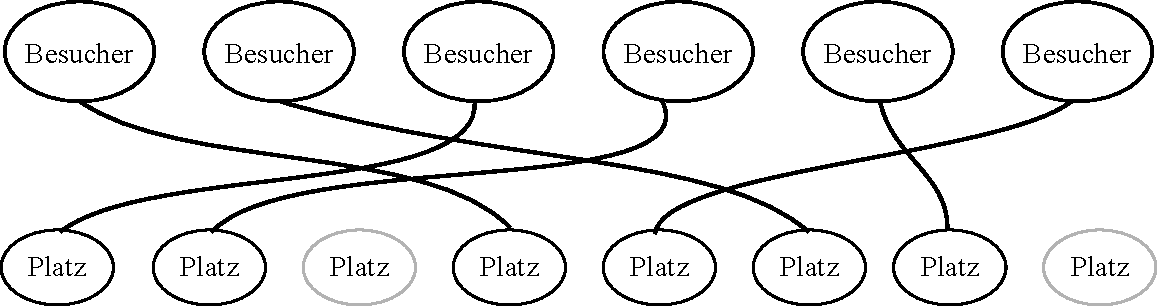
\includegraphics[scale=0.5]{Kinoabbildungen.pdf}
	\end{figure}

	\textbf{Achtung:} Das dient nur der Veranschaulichung und ist \textbf{keine} Möglichkeit, eine Abbildung formal anzugeben!
\end{frame}

%\begin{frame}
%	\frametitle{Lösung}
%	\textit{In dieser Teilaufgabe nehmen wir an, 6 Kinobesucher besuchten ein Kino mit 8 Plätzen. Wie viele injektive Abbildungen gibt es?} \\[2em] \pause
%	
%	Es gibt insgesamt $$8 \cdot 7 \cdot 6 \cdot 5 \cdot 4 \cdot 3 = 20160$$ injektive Abbildungen. \\[1em]
%	Der erste Besucher hat 8 Plätze zur Auswahl. Da aufgrund der Injektivität der nächste Besucher einen anderen Sitzplatz wählen muss, stehen ihm noch 7 Plätze zur Auswahl. Dies kann man für die restlichen Besucher fortsetzen.
%	
%\end{frame}

\subsection{Aufgabe 2}
\begin{frame}{Aufgabe 2}
	
	Was kann man über die Surjektivität, Injektivität und Bijektivität folgender Abbildungen sagen? Begründet jeweils kurz.
	\visible<+(-1)>{}
	\begin{alist}
		\item $f \from \R \functionto \R, \; x \mapsto x^2$ \\
		\visible<+-|handout:2->{
			Weder injektiv ($f(-2) = f(2) = 4$) noch surjektiv (auf $-1 \in \R$ wird nicht abgebildet) \impl auch nicht bijektiv.
		}
		\item $f \from \R_+ \functionto \R_+, \; x \mapsto x^2$ \\
		\visible<+-|handout:2->{
			Wir können zu jedem $y \in \R_+$ ein $x \in \R_+$ angeben, so dass $f(x) = y$, nämlich $ x = \sqrt{\mathstrut y}$. \\
			\impl surjektiv, und da dieses $x$ eindeutig ist auch injektiv \impl bijektiv.
		}
		
		\item $f \from \N_0 \functionto \N_0, \; x \mapsto \casesl{ 42 & \text{wenn $x = 0$} \\ x - 1 & \text{sonst} }$ \\
		\visible<+-|handout:2->{
			Nicht injektiv ($f(0) = f(43) = 42$), aber surjektiv (Für jedes $x \in \N_0$ gilt: $x + 1 \in \N_0 \text{ und } f(x+1) = x$) \\ \impl nicht bijektiv.
		} 
	\end{alist}
\end{frame}



%\begin{frame}[t]
%	\begin{block}{Wahr oder Falsch?}
%		Sei $M$ eine beliebige endliche Menge und $f$ eine Abbildung $f \from M \functionto M$. \\
%			\TrueQuestion{Wenn $f$ injektiv ist, dann ist $f$ auch surjektiv.}
%			\TrueQuestion{Wenn $f$ surjektiv ist, dann ist $f$ auch injektiv.}
%			\FalseQuestionE{Die beiden Aussagen gelten auch, wenn $M$ nicht endlich ist.}{Gegenbeispiele: \\ 
%				$f \from \N_0 \functionto \N_0, n \mapsto 2 \* n $ \\ 
%				$g \from \N_0 \functionto \N_0, n \mapsto \floor{\dfract n/2 }$}
%	\end{block}
%	
%\end{frame}

\begin{frame}[t]{Injektivität und Surjektivität}
	Was bedeutet nochmal injektiv und surjektiv?
	\begin{itemize}
		\item Eine Funktion $ f \from M \functionto N $ heißt \textit{injektiv} wenn gilt: \\
			\pause
			für alle $m_1,m_2 \in M$ gilt: Aus $ f(m_1)=f(m_2) $ folgt $ m_1 = m_2 $
		\pause
		\item Eine Funktion $ f \from M \functionto N $ heißt \textit{surjektiv} wenn gilt: \\
			\pause
			für alle $n \in N$ existiert ein $m \in M$ sodass $f(m)=n$ gilt
	\end{itemize}
	\pause
	\begin{block}{Wahr oder Falsch?}
		Sei $M$ eine beliebige endliche Menge und $f$ eine Abbildung $f \from M \functionto M$. \\
			\TrueQuestion{Wenn $f$ injektiv ist, dann ist $f$ auch surjektiv.}
			\TrueQuestion{Wenn $f$ surjektiv ist, dann ist $f$ auch injektiv.}
			\FalseQuestionE{Die beiden Aussagen gelten auch, wenn $M$ nicht endlich ist.}{Gegenbeispiele: \\ 
				$f \from \N_0 \functionto \N_0, n \mapsto 2 \* n $ \\ 
				$g \from \N_0 \functionto \N_0, n \mapsto \floor{\dfract n/2 }$}
	\end{block}
\end{frame}

\section{Wörter}

\begin{frame}{Wörter}
	\begin{block}{Definition}
		\begin{itemize}
			\item Ein \textbf{Alphabet} $A$ ist eine endliche, nichtleere Menge von Zeichen. \pause
			\item Ein \textbf{Wort} $w$  über einem Alphabet $A$ ist ein \textbf{endliche Folge von Zeichen} aus A \\ 
		\end{itemize}
	\end{block}	
	
	\pause
	\begin{block}{Definition}
		$A^*$ ist die \textbf{Menge aller Wörter} beliebiger Länge, die nur Zeichen aus $A$ enthalten.
		% brauchen wir das?
		\mycomment{, also:\\
		\pause 
		$A^*$ ist die Menge aller Abbildungen $w \from \Z_n \functionto B$ mit $n \in \N_0$ und $B \subseteq A$. \\}
	\end{block}

	\pause
	\begin{block}{Beispiel}
		Sei $ A = \{ \word a, \word b \} $ ein Alphabet. 
		Dann sind $ w_1 = \word{aabbabab}$ und $w_2 = \word{ab} $ zwei mögliche Wörter über $A$. 
		\impl $ w_1 \in A^*, w_2 \in A^*$
	\end{block}

\end{frame}

\begin{frame}{Wörter -- \thassedaniel{formal betrachtet}{Formalkram}}
	\begin{block}{Formale Definition}
		Ein \textbf{Wort} $w$  über einem Alphabet $A$ ist eine \textit{surjektive} Abbildung $w \from \Z_n \functionto B$ mit $B \subseteq A$. \\ 
		\smallskip
		Zur Erinnerung: \; $ \Z_n = \{i \in \N_0 \mid 0 \leq i < n \} = \set{0, ..., n-1} $ 
	\end{block}
	
	\begin{block}{Beispiel}
		Sei $ A := \{ \word a, ..., \word z \} $ ein Alphabet und $B := \set{\word a, \word b, \word e, \word n, \word o, \word r, \word s, \word t} \subseteq A$. \\
		Dann ist ein Wort $w$ gegeben durch $ w \from \Z_{12} \functionto B$, \\ 
		\smallskip
		\begin{tabular}{c|c@{\:}c@{\:}c@{\:}c@{\:}c@{\:}c@{\:}c@{\:}c@{\:}c@{\:}c@{\:}c@{\:}c@{\:}c@{\:}c@{\:}c}
			$i$ & \small 0 & \small 1 & \small 2 & \small 3 & \small 4 & \small 5 & \small 6 & \small 7 & \small 8 & \small 9 & \small 10 & \small 11 \\
			\hline
			$w(i)$ & \word a & \word n & \word a & \word n & \word a & \word s & \word s & \word o & \word r & \word b & \word e & \word t 
		\end{tabular} \\
		\bigskip
		Oder einfach wie vorhin: \quad  $w := \word{ananassorbet}$.
	\end{block}
\end{frame}

\begin{frame}[t]{Das leere Wort}
	\begin{block}{Definition}
		Wir definieren das \textbf{leere Wort} als $$ \varepsilon \from \Z_0  \functionto \set{} \qquad\text{bzw.}\qquad \eps \from \set{} \functionto \set{} $$ \pause

	\end{block}
	
	\begin{block}{Wichtig}
		Das leere Wort ist \textbf{nicht} Nichts, sondern ein echtes Wort! \\
		($0 \in \N_0$ ist ja auch ne Zahl! $\emptyset$ ist auch ne Menge!)
	\end{block}
		%Wichtig: Das leere Wort ist auch ein \enquote{echtes, gleichberechtigtes} Wort. Die Null ist bei den natürlichen Zahlen ja auch nicht einfach \enquote{nichts}. \medskip \pause
		
		\YesQuestionE{Ist $\eps \from \set{} \functionto \set{} $ eine Relation? Und eine Funktion? Ist es surjektiv?}{
			Achtung: Wir müssen fordern, dass Wörter surjektiv sind, sonst ist das leere Wort nicht eindeutig!
		}
	
\end{frame}


\begin{frame}[t]{Konkatenation von Wörtern}
	\begin{block}{Wörter „aneinanderkleben“}
		Seien $w_1 = \word{erd}, w_2 = \word{blumentopf}$. \\
		Dann ist $ w_1 \* w_2 = \word{erdblumentopf} \neq w_2 \* w_1 = \word{blumentopferd}$. \\ 
		\pause
		Konkatenation ist also \textbf{nicht kommutativ!} \\
		\YesQuestionE{Ist sie \textbf{assoziativ}?}{$(w_1 \* w_2) \* w_3 = w_1 \* (w_2 \* w_3)$.} \medskip 
		\only<+->{Außerdem gilt immer $ \eps \* w \* \eps = w $.}
		
	\end{block}
	
	
	\visible<+->{
		\begin{block}{Beobachtung}
			Falls $w=w_1\* w_2 $ und $w_1 \in A^* , w_2 \in B^* $, dann ist
			$ w\in (A \cup B)^* $.
		\end{block}
	
		\begin{block}{„Wortpotenzen“}
			\vspace{-2\baselineskip}
			\begin{align*}
				w^0 &= \eps \\
				w^k &= \underbrace{w \* w  \cdots  w}_{\text{$k$-mal}}
			\end{align*}
	
		\end{block}
	}

\end{frame}

\begin{frame}{Länge von Wörtern}
	\begin{block}{Definition}
		$\size w$: Die \textbf{Länge} eines Wortes $w$, also die Gesamtanzahl der Zeichen von $w$.
	\end{block}
	
	\begin{block}{Beispiel}
		$$ \size{\word{hallo}} = 5 \qqquad \size \eps = 0$$
	\end{block}

	\pause
	\begin{block}{Lemmata}
		$$ \size{a \* b} = \size a + \size b $$ \\
		\pause
		$$ \size{w^k} = k \* \size w $$
	\end{block}

\end{frame}

\begin{frame}{Wörter}
	\begin{block}{Definition}
		$A^n$: \emph{Menge aller Wörter der Länge $n$} über dem Alphabet $A$.\\
		Wie kann man damit $A^*$ ausdrücken? \\
		\pause
		\[ A^* = \bigcup \limits_{i = 0}^\infty A^i \]
	\end{block}
	
	
	\pause
	\begin{block}{Erinnerung}
		$
		\bigcup \limits_{i\in I} M_i = \{ x \mid \text{es gibt ein } i\in I \text{ so, dass } x\in  M_i \}  
		$
	\end{block}
\end{frame}

\begin{frame}{Aufgabe 3}
	\visible<+(-1)>{}
	\begin{itemize}
		\item Welche Wörter lassen sich aus dem Alphabet $A = \{ \word a , \word b \}$ bilden? Was enthält die Menge $A^*$? \\
		\visible<+-|handout:2->{
			\impl $\word a, \word b, \word {aa}, \word {bb}, \word {ab}, \word {ba}, \word {aaa}, \word {bbb}, \dots$ \\
			\impl $A^*$ enthält genau diese Wörter (und auch $\eps$!).
		}
		\item Ist das Wort $w = \word{aabb} \* \word{ba}$ ein Element der Menge $A^5$? \\
		\visible<+-|handout:2->{
			\impl Nein. $w = \word{aabbba}$ ist zwar ein Wort über $A$, aber hat Länge $6 \neq 5$.
		}
		\item Was ist $A^2 \times A^2$? \\
			\visible<+-|handout:2->{
				\impl $ A^2 \times A^2 = \set{(\word{aa},\word {aa}),(\word{aa},\word{bb}),(\word {aa},\word {ab}),(\word {aa},\word {ba}),(\word {bb},\word {aa}), \dots }$
			} \\ \smallskip
			Wir definieren die Abbildung $f \from A^* \times A^* \functionto A^*, \; (w_1, w_2) \mapsto w_1 \cdot w_2$. \\
			Was ist $f(A^2 \times A^2)$? \\
			\uncover<+-|handout:2->{
				\impl $ f(A^2 \times A^2) = \set{\word{aaaa}, \word{aabb}, \word{aaab}, \word{aaba}, \word{bbaa}, \dots } = A^4 $
			}\\
		\bigskip
		Erinnerung: Für $f \from A \functionto B, M \subseteq A$ definieren wir $f(M) = \{f(a) \mid a \in M\}$
	\end{itemize}
\end{frame}




\begin{frame}	
	\begin{block}{Was ihr nun wissen solltet}
		\begin{itemize}
			\item Wie und wo ihr euer Übungsblatt \textbf{ab sofort} abgebt
			\item Welche Eigenschaften Relationen und Funktionen haben können
			\item Was Alphabete und Wörter sind
			\item Wie man mit Wörtern rechnet
		\end{itemize}
	\end{block}
	
	\begin{block}{Was nächstes Mal kommt}
		\begin{itemize}
			\item Sinnvollere Gebilde als \word{\thassedaniel{egnarts\sp si\sp efiL}{retsinnaL\sp nosrO}} mit \emph{formalen Sprachen}
			\item Aus Sage wird Logik: \emph{Aussagenlogik}
		\end{itemize}
	\end{block}
\end{frame}

\xkcdframe{1121}{Danke für eure Aufmerksamkeit! \smiley}{1.5}
\slideThanks

\end{document}